%% ============================================================
%%  Relatório IAM TP — MEI, Gestão de Identidade — ESTG-IPP
%%  2025/2026 — Avelino Almeida (8220800@estg.ipp.pt)
%%  Formato: template ESTG-P.Porto (report class)
%% ============================================================
\documentclass[12pt,a4paper,twoside]{report}

%% ---- Codificação e Língua ----
\usepackage[utf8]{inputenc}
\usepackage[portuguese]{babel}

%% ---- Layout ----
\usepackage[margin=2.5cm]{geometry}

%% ---- Índices ----
\usepackage[nottoc,numbib]{tocbibind}

%% ---- PDF Capa ----
\usepackage{pdfpages}

%% ---- Parágrafo ----
\usepackage{parskip}

%% ---- URLs ----
\usepackage{url}

%% ---- Acrónimos ----
\usepackage[acronym]{glossaries}
\makeglossaries

%% ---- Listagens de código ----
\usepackage{listings}
\renewcommand{\lstlistingname}{Listagem}
\renewcommand*{\lstlistlistingname}{Lista de Listagens}
\lstset{
  xleftmargin  = 1cm,
  basicstyle   = \footnotesize\ttfamily,
  numbers      = left,
  captionpos   = b,
  columns      = fullflexible,
  breaklines   = true,
  frame        = single,
  showstringspaces = false
}

%% ---- Gráficos e Figuras ----
\usepackage{graphicx}
\usepackage{float}
\usepackage{caption}
\graphicspath{{../imagens/}}

%% ---- Tabelas ----
\usepackage{booktabs}
\usepackage{tabularx}
\usepackage{array}
\usepackage[table,xcdraw]{xcolor}
\usepackage{longtable}

%% ---- Hiperligações ----
\usepackage[colorlinks=true, linkcolor=black, citecolor=black, urlcolor=blue]{hyperref}

%% ---- Outros ----
\usepackage{enumitem}

%% ============================================================
\begin{document}

%% ---- CAPA (substituir pelo ficheiro oficial quando disponível) ----
%% \includepdf[pages=1-2]{capas/capa.pdf}
%% ============================================================
%%  Capa Manual (usar \includepdf quando capa.pdf disponível)
%% ============================================================
\begin{titlepage}
  \thispagestyle{empty}
  \centering
  \vspace*{1.5cm}

  {\large\bfseries Instituto Politécnico do Porto}\\[0.3cm]
  {\large Escola Superior de Tecnologia e Gestão}\\[0.5cm]
  {\normalsize Mestrado em Engenharia Informática}\\[2.5cm]

  \rule{\linewidth}{1.2pt}\\[0.5cm]
  {\huge\bfseries Plataforma de Gestão de\\[0.3cm]Identidade e Acesso}\\[0.5cm]
  {\Large\bfseries com Keycloak, FastAPI e Docker}\\[0.5cm]
  \rule{\linewidth}{1.2pt}\\[1.5cm]

  {\large Relatório do Trabalho Prático}\\[0.3cm]
  {\normalsize Unidade Curricular: Gestão de Identidade}\\[0.2cm]
  {\normalsize Docente: Ricardo Costa}\\[2cm]

  {\large\bfseries Autores:}\\[0.5cm]
  {\large Avelino Almeida — 8220800}\\[0.2cm]
  {\normalsize 8220800@estg.ipp.pt}\\[2cm]

  {\normalsize Ano letivo: 2025/2026}\\[0.3cm]
  {\normalsize Entrega/Demo: 28 de maio de 2026}

  \vfill
  {\small MEI-GI · ESTG-IPP · 2025/2026}
\end{titlepage}


\pagenumbering{roman}

%% ---- ACRÓNIMOS ----
%% ============================================================
%%  Acrónimos — Projeto IAM — MEI-GI ESTG-IPP 2025/2026
%% ============================================================

\newacronym{iam}{IAM}{Identity and Access Management}
\newacronym{idp}{IdP}{Identity Provider}
\newacronym{oidc}{OIDC}{OpenID Connect}
\newacronym{oauth2}{OAuth 2.0}{Open Authorization 2.0}
\newacronym{jwt}{JWT}{JSON Web Token}
\newacronym{jwks}{JWKS}{JSON Web Key Set}
\newacronym{rbac}{RBAC}{Role-Based Access Control}
\newacronym{mfa}{MFA}{Multi-Factor Authentication}
\newacronym{totp}{TOTP}{Time-based One-Time Password}
\newacronym{otp}{OTP}{One-Time Password}
\newacronym{jml}{JML}{Joiner-Mover-Leaver}
\newacronym{api}{API}{Application Programming Interface}
\newacronym{rest}{REST}{Representational State Transfer}
\newacronym{json}{JSON}{JavaScript Object Notation}
\newacronym{pkce}{PKCE}{Proof Key for Code Exchange}
\newacronym{ropc}{ROPC}{Resource Owner Password Credentials}
\newacronym{acl}{ACL}{Access Control List}
\newacronym{siem}{SIEM}{Security Information and Event Management}
\newacronym{saml}{SAML}{Security Assertion Markup Language}
\newacronym{uri}{URI}{Uniform Resource Identifier}
\newacronym{http}{HTTP}{HyperText Transfer Protocol}
\newacronym{https}{HTTPS}{HyperText Transfer Protocol Secure}
\newacronym{tls}{TLS}{Transport Layer Security}
\newacronym{cli}{CLI}{Command Line Interface}
\newacronym{spa}{SPA}{Single Page Application}
\newacronym{mei}{MEI}{Mestrado em Engenharia Informática}
\newacronym{estg}{ESTG}{Escola Superior de Tecnologia e Gestão}
\newacronym{ipp}{IPP}{Instituto Politécnico do Porto}
\newacronym{ui}{UI}{User Interface}
\newacronym{ux}{UX}{User Experience}


%% ---- DECLARAÇÃO DE INTEGRIDADE ----
\chapter*{Declaração de Integridade}
\addcontentsline{toc}{chapter}{Declaração de Integridade}

Eu, \textbf{Avelino Almeida}, estudante nº \textbf{8220800}, do Mestrado em \textbf{Engenharia Informática} da Escola Superior de Tecnologia e Gestão do Instituto Politécnico do Porto, declaro que não fiz plágio nem auto-plágio, pelo que o trabalho intitulado \textbf{``Plataforma de Gestão de Identidade e Acesso com Keycloak, FastAPI e Docker''} é original e da minha autoria, não tendo sido usado previamente para qualquer outro fim. Mais declaro que todas as fontes usadas estão citadas, no texto e na bibliografia final, segundo as regras de referenciação adotadas na instituição.

\vspace{1.5cm}
\noindent Porto, 28 de maio de 2026

\vspace{1cm}
\noindent\rule{7cm}{0.4pt}\\
Avelino Almeida

%% ---- AGRADECIMENTOS ----
\chapter*{Agradecimentos}
\addcontentsline{toc}{chapter}{Agradecimentos}

Agradeço ao docente Ricardo Costa pela orientação e pelos materiais disponibilizados ao longo da unidade curricular de Gestão de Identidade, que permitiram aprofundar os conhecimentos teóricos e práticos em \gls{iam}.

Agradeço igualmente à comunidade de código aberto do projeto Keycloak, cujas ferramentas e documentação tornaram possível a implementação de uma solução \gls{iam} completa e robusta sem custos de licença.

%% ---- ABSTRACT ----
\chapter*{Abstract}
\addcontentsline{toc}{chapter}{Abstract}

This report describes the design and implementation of a complete \textit{Identity and Access Management} (IAM) platform, developed as the practical assignment for the Identity Management course (MEI, ESTG-IPP, 2025/2026).

The fully containerised solution combines \textbf{Keycloak~26} as the central Identity Provider (IdP), a \textbf{FastAPI} (Python~3.12) application as the protected resource server, and \textbf{PostgreSQL~16} as the persistence backend — all orchestrated by Docker Compose. The platform demonstrates: federated authentication via \gls{oidc}/\gls{oauth2} with \gls{jwt} RS256 validation, Role-Based Access Control (\gls{rbac}) with three hierarchical profiles, mandatory \gls{mfa}/\gls{totp} for administrators, the full Joiner–Mover–Leaver (\gls{jml}) identity lifecycle via the Keycloak Admin \gls{rest} \gls{api}, and comprehensive event auditing.

The entire infrastructure is reproduced with a single \texttt{docker compose up --build} command. An interactive dashboard provides live evidence for all requirements.

\textbf{Keywords:} Identity Management, Keycloak, OIDC, OAuth~2.0, JWT, RBAC, MFA, TOTP, JML, FastAPI, Docker.

%% ---- RESUMO ----
\chapter*{Resumo}
\addcontentsline{toc}{chapter}{Resumo}

Este relatório descreve a conceção e implementação de uma plataforma completa de Gestão de Identidade e Acesso (\gls{iam}), desenvolvida no âmbito do trabalho prático da unidade curricular de Gestão de Identidade (MEI, ESTG-IPP, 2025/2026).

A solução containerizada combina o \textbf{Keycloak~26} como \gls{idp} central, uma \gls{api} \textbf{FastAPI} (Python~3.12) como servidor de recursos protegido e \textbf{PostgreSQL~16} como base de dados de suporte — todos orquestrados por Docker Compose. O projeto demonstra: autenticação federada via \gls{oidc}/\gls{oauth2} com validação de \gls{jwt} RS256, controlo de acesso baseado em papéis (\gls{rbac}) com três perfis hierárquicos, \gls{mfa}/\gls{totp} obrigatória para administradores, o ciclo de vida completo \gls{jml} via Keycloak Admin \gls{rest} \gls{api}, e auditoria completa de eventos.

Toda a infraestrutura é reproduzida com um único comando (\texttt{docker compose up --build}) e um dashboard interativo fornece evidência em direto de todos os requisitos.

\textbf{Palavras-chave:} Gestão de Identidade, Keycloak, OIDC, OAuth~2.0, JWT, RBAC, MFA, TOTP, JML, FastAPI, Docker.

%% ---- ÍNDICES ----
\tableofcontents
\listoffigures
\listoftables
\addcontentsline{toc}{chapter}{Lista de Listagens}
\lstlistoflistings
\printglossary[type=\acronymtype, title=Acrónimos, nonumberlist]

%% ============================================================
%%  CAPÍTULOS
%% ============================================================
\pagenumbering{arabic}

%% ============================================================
%%  Capítulo 1 — Introdução
%% ============================================================
\chapter{Introdução}
\label{chap:introducao}

\section{Contexto e Motivação}

A gestão de identidades e acessos (\gls{iam}) constitui um dos pilares fundamentais da segurança empresarial moderna. À medida que as organizações adotam arquiteturas distribuídas, serviços em nuvem e modelos de trabalho híbrido, a necessidade de um sistema centralizado que gira \textit{quem} pode aceder a \textit{quê}, \textit{quando} e \textit{como} torna-se crítica \cite{NIST80063B}.

Sem um \gls{iam} robusto, as organizações ficam expostas a riscos como acesso não autorizado a recursos sensíveis, proliferação de credenciais não geridas, incapacidade de revogar acessos em tempo real e ausência de rastreabilidade de eventos de segurança. A adoção de um \gls{idp} centralizado, aliado a protocolos de autenticação padronizados (\gls{oidc}, \gls{oauth2}) e a políticas de autorização bem definidas (\gls{rbac}), mitiga estes riscos de forma sistemática.

\section{Objetivos}

Este trabalho prático da UC de Gestão de Identidade tem como objetivo consolidar os conceitos de identidade digital e ciclo de vida (\gls{jml}), autenticação e federação, autorização e controlo de acessos, \gls{mfa} e auditoria e segurança operacional \cite{Costa2026}.

Os objetivos específicos são:

\begin{enumerate}
  \item Configurar um \gls{idp} centralizado com Keycloak~26, incluindo \textit{realm} dedicado, pelo menos 3 perfis como \textit{realm roles}/\textit{groups}, clientes \gls{oidc} e estrutura de utilizadores;
  \item Implementar autenticação \gls{oidc}/\gls{oauth2} com validação local de \gls{jwt} RS256 via \gls{jwks} e obtenção de \textit{claims} básicas;
  \item Aplicar controlo de acesso \gls{rbac} com prova de permitir/negar por papel em endpoints de uma \gls{api} \gls{rest};
  \item Ativar e demonstrar \gls{mfa} \gls{totp} obrigatória, incluindo evidência do fluxo de configuração;
  \item Implementar os três fluxos \gls{jml} via Keycloak Admin \gls{rest} \gls{api} com impacto imediato no acesso;
  \item Registar e disponibilizar evidência consultável de eventos críticos de auditoria, incluindo um excerto no relatório;
  \item Containerizar toda a infraestrutura com Docker Compose e fornecer \texttt{realm-export.json} para reprodutibilidade.
\end{enumerate}

\section{Caso de Uso}

O cenário implementado simula uma \textbf{aplicação interna empresarial} com três perfis de utilizador: \textbf{visitante} (acesso a recursos públicos e perfil próprio), \textbf{colaborador} (acesso a dados e funcionalidades internas) e \textbf{administrador} (acesso total, incluindo gestão de utilizadores, auditoria e áreas protegidas por \gls{mfa}).

\section{Estrutura do Relatório}

Este relatório está organizado da seguinte forma:
\begin{itemize}
  \item Capítulo~\ref{chap:estado_arte} — Estado da Arte em \gls{iam} e protocolos relevantes;
  \item Capítulo~\ref{chap:trabalho_relacionado} — Análise de soluções \gls{iam} alternativas;
  \item Capítulo~\ref{chap:desenho} — Arquitetura e decisões técnicas de implementação;
  \item Capítulo~\ref{chap:validacao} — Validação, testes e resultados obtidos;
  \item Capítulo~\ref{chap:conclusao} — Conclusões e trabalho futuro.
\end{itemize}

<<<<<<< HEAD
%% Capítulo 2 — Estado da Arte
\chapter{Estado da Arte}
\label{chap:estado_arte}

\textbf{OIDC / OAuth~2.0} — O \gls{oauth2} \cite{RFC6749} é a \textit{framework} de autorização padrão da indústria. O \gls{oidc} \cite{OIDCCore} acrescenta uma camada de identidade, introduzindo o \textit{ID Token} e o \textit{UserInfo Endpoint}. O fluxo recomendado para aplicações \textit{web} é \textit{Authorization Code com PKCE} \cite{RFC7636}; em testes usa-se \gls{ropc}.

\textbf{JWT e JWKS} — O \gls{jwt} \cite{RFC7519} é um token compacto com três partes (header, payload, signature) codificadas em Base64URL. O algoritmo RS256 usa criptografia assimétrica: o \gls{idp} assina com a chave privada e os \textit{resource servers} validam localmente com a chave pública obtida via \gls{jwks} \cite{RFC7517}, sem chamadas adicionais ao \gls{idp}.

\textbf{RBAC} — O \gls{rbac} \cite{Ferraiolo1992} associa permissões a papéis; os utilizadores herdam permissões por atribuição de papel. Simplifica a administração face a listas de controlo de acesso (\gls{acl}) e é adequado para a maioria dos cenários empresariais.

\textbf{MFA / TOTP} — A \gls{mfa} \cite{NIST80063B} exige dois ou mais fatores independentes. O \gls{totp} \cite{RFC6238} gera códigos de 6 dígitos, válidos 30 segundos, baseados numa chave partilhada e no \textit{timestamp}. O NIST SP~800-63B recomenda AAL2 (com \gls{mfa}) para acesso a dados sensíveis.

\textbf{JML} — O ciclo de vida Joiner–Mover–Leaver \cite{IDPro} automatiza o provisionamento, a transição e a revogação de acessos, eliminando contas órfãs e garantindo o princípio do privilégio mínimo em cada fase.
=======
%% ============================================================
%%  Capítulo 2 — Estado da Arte
%% ============================================================
\chapter{Estado da Arte}
\label{chap:estado_arte}

\section{Gestão de Identidade e Acesso}

A \gls{iam} é o conjunto de políticas, processos e tecnologias que garante que os utilizadores certos têm acesso aos recursos certos, no momento certo e pelos motivos certos \cite{NIST80063B}. Os pilares de um sistema \gls{iam} são:

\begin{itemize}
  \item \textbf{Autenticação}: verificar a identidade declarada pelo utilizador;
  \item \textbf{Autorização}: determinar o que o utilizador pode fazer;
  \item \textbf{Gestão do ciclo de vida}: criar, atualizar e desativar identidades de forma controlada;
  \item \textbf{Auditoria}: registar eventos para rastreabilidade, conformidade e deteção de ameaças.
\end{itemize}

\section{OpenID Connect e OAuth 2.0}

O \gls{oauth2} \cite{RFC6749} é uma \textit{framework} de autorização que permite que aplicações obtenham acesso limitado a contas de utilizadores, sem expor as credenciais. O \gls{oidc} \cite{OIDCCore} acrescenta uma camada de identidade sobre \gls{oauth2}, introduzindo o conceito de \textit{ID Token} e o \textit{UserInfo Endpoint}, que permitem que clientes verifiquem a identidade do utilizador e obtenham informação de perfil básica.

Os fluxos \gls{oidc} mais relevantes são:
\begin{itemize}
  \item \textbf{Authorization Code com PKCE} \cite{RFC7636} — recomendado para aplicações \textit{web} e \textit{mobile}; o \gls{pkce} protege contra ataques de interceção do código de autorização;
  \item \textbf{Resource Owner Password Credentials} (\gls{ropc}) — utilizado apenas em testes e ambientes controlados; transmite credenciais diretamente ao servidor de autorização.
\end{itemize}

\section{JSON Web Token (JWT)}

O \gls{jwt} \cite{RFC7519} é um standard aberto que define um método compacto para transmitir informação entre partes como um objeto \gls{json} verificável. É composto por três partes codificadas em Base64URL: \textit{header} (algoritmo), \textit{payload} (\textit{claims}) e \textit{signature}.

O algoritmo \textbf{RS256} utiliza criptografia assimétrica: o \gls{idp} assina com a chave privada e os \textit{resource servers} validam com a chave pública. A distribuição segura das chaves públicas é feita via \gls{jwks} \cite{RFC7517} — um \textit{endpoint} \gls{json} que publica o conjunto de chaves ativas do \gls{idp}.

\section{Controlo de Acesso Baseado em Papéis (RBAC)}

O \gls{rbac} \cite{Ferraiolo1992} é um modelo de controlo de acesso em que as permissões são associadas a \textbf{papéis}, e os utilizadores adquirem permissões ao serem atribuídos a esses papéis. Este modelo simplifica a administração em comparação com listas de controlo de acesso (\gls{acl}) e é adequado para a maioria dos cenários empresariais.

O NIST define quatro modelos \gls{rbac} progressivos: \textit{Core RBAC}, \textit{Hierarchical RBAC}, \textit{Constrained RBAC} e \textit{Symmetric RBAC}. Neste projeto adota-se o \textit{Core RBAC} com elementos de hierarquia implícita (o papel \texttt{admin} acede a tudo o que o \texttt{colaborador} acede).

\section{Autenticação Multifator (MFA) e TOTP}

A \gls{mfa} \cite{NIST80063B} exige que o utilizador prove a sua identidade com dois ou mais fatores independentes: \textit{algo que sabe} (password), \textit{algo que tem} (dispositivo \gls{totp}) e/ou \textit{algo que é} (biometria).

O \gls{totp} \cite{RFC6238} gera códigos numéricos temporários baseados numa chave partilhada (\textit{secret}) e no \textit{timestamp} atual. A especificação define uma janela de 30 segundos e códigos de 6 dígitos, compatível com Google Authenticator, Microsoft Authenticator e Authy.

O NIST SP~800-63B classifica os autenticadores em três níveis (\textit{Authentication Assurance Levels} — AAL1, AAL2, AAL3) e recomenda AAL2 (com \gls{mfa}) para acesso a dados sensíveis.

\section{Ciclo de Vida de Identidades — JML}

O ciclo de vida \gls{jml} refere-se aos três processos chave de gestão de identidades empresariais \cite{IDPro}:

\begin{itemize}
  \item \textbf{Joiner} (\textit{Integração}): provisionar o acesso inicial quando um utilizador entra na organização ou muda de função — o princípio do \textit{least privilege} deve ser aplicado desde o início;
  \item \textbf{Mover} (\textit{Transição}): ajustar os acessos quando um utilizador muda de papel ou departamento — a revogação do acesso anterior deve ser imediata;
  \item \textbf{Leaver} (\textit{Saída}): desprovisionar todos os acessos quando um utilizador sai — contas órfãs são um vetor de ataque crítico.
\end{itemize}

A automação destes processos através de \gls{api}s de administração (como a Keycloak Admin \gls{rest} \gls{api}) elimina o erro humano e garante consistência.
>>>>>>> df2eb5220b31d8e704cf4f670cff764b26edabce

%% Capítulo 3 — Trabalho Relacionado
\chapter{Trabalho Relacionado}
\label{chap:trabalho_relacionado}

A Tabela~\ref{tab:comparacao_iam} compara as principais soluções \gls{iam} consideradas.

\begin{table}[h!]
\centering
\caption{Comparação de soluções IAM}
\label{tab:comparacao_iam}
\begin{tabularx}{\textwidth}{|l|l|X|X|}
\hline
\textbf{Solução} & \textbf{Modelo} & \textbf{Pontos fortes} & \textbf{Limitações} \\ \hline
Auth0 & SaaS & Fácil integração, documentação extensa & Custo elevado, dependência de terceiro \\ \hline
Azure AD B2C & Cloud & Integração Microsoft, escala empresarial & Configuração complexa, custo por login \\ \hline
Okta & SaaS & UX excelente, \gls{mfa} avançada & Licenciamento por utilizador \\ \hline
\textbf{Keycloak} & Open Source & \textbf{Gratuito, self-hosted, Admin API completa} & Curva de aprendizagem \\ \hline
\end{tabularx}
\end{table}

O \textbf{Keycloak~26} \cite{KeycloakDocs} foi escolhido por: custo zero; execução local via Docker; \texttt{realm-export.json} versionável; suporte nativo a \gls{mfa} \gls{totp}; Admin \gls{rest} \gls{api} para automação \gls{jml}; e revogação de sessões com efeito imediato via \texttt{DELETE /users/\{id\}/sessions}.

Relativamente à validação de tokens, optou-se por \textbf{validação local via \gls{jwks}} (em vez de \textit{token introspection}) para eliminar latência e dependência de disponibilidade do \gls{idp} em cada pedido, compensando a limitação de revogação imediata através da revogação explícita de sessões nos fluxos \gls{jml}.

%% ============================================================
%%  Capítulo 4 — Desenho e Especificação
%% ============================================================
\chapter{Desenho e Especificação}
\label{chap:desenho}

\section{Arquitetura do Sistema}

A arquitetura segue o padrão \textbf{Resource Server + Identity Provider}, com separação clara de responsabilidades entre os três serviços orquestrados por Docker Compose.

\begin{figure}[h!]
  \centering
  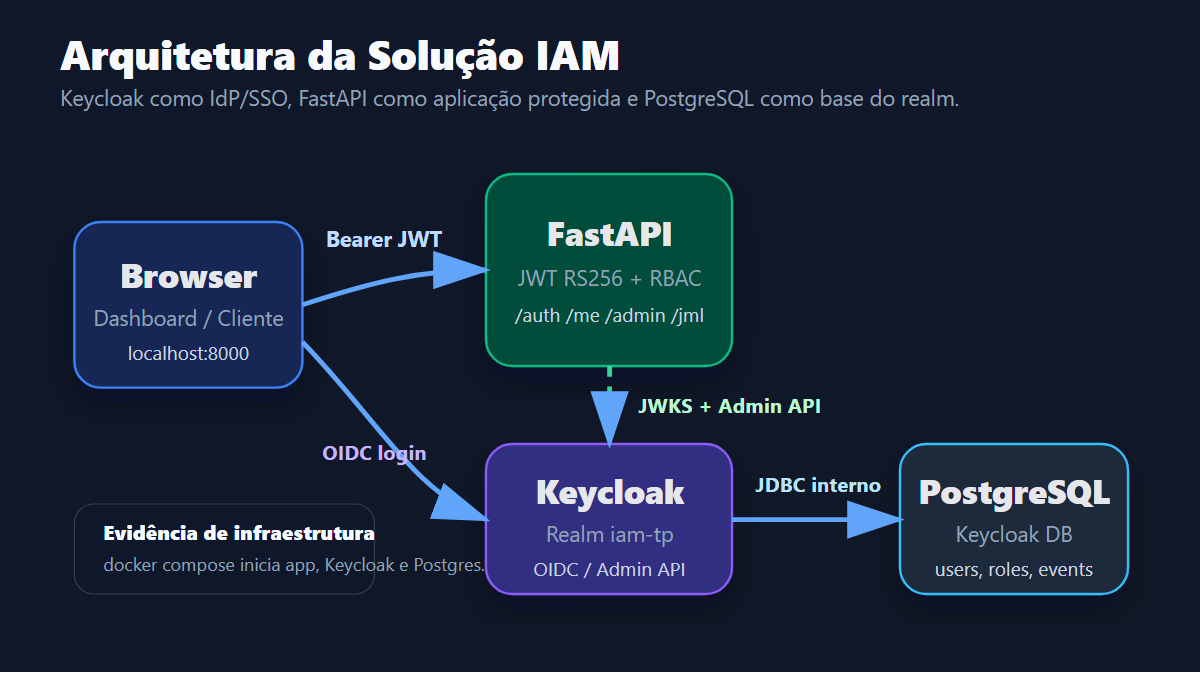
\includegraphics[width=0.95\textwidth]{arquitetura_iam.png}
  \caption{Arquitetura do projeto: FastAPI, Keycloak 26 e PostgreSQL 16 sob Docker Compose.}
  \label{fig:arquitetura}
\end{figure}

O fluxo principal, ilustrado na Figura~\ref{fig:arquitetura}, é: (1)~o cliente autentica no Keycloak e recebe um \gls{jwt} assinado com RS256; (2)~apresenta o token à FastAPI; (3)~a FastAPI valida a assinatura localmente via \gls{jwks} cacheado; (4)~aplica \gls{rbac}; (5)~responde ao cliente.

\begin{table}[h!]
\centering
\caption{Componentes da arquitetura, portos e funções}
\label{tab:componentes}
\begin{tabular}{|l|c|l|}
\hline
\textbf{Componente} & \textbf{Porto} & \textbf{Função principal} \\ \hline
Keycloak~26 & 8081 & \gls{idp}: emissão de \gls{jwt}, realm, \gls{rbac}, \gls{mfa}, auditoria \\ \hline
FastAPI (Python~3.12) & 8000 & \textit{Resource server}: validação \gls{jwt}, endpoints protegidos, dashboard \\ \hline
PostgreSQL~16 & 5432 & Base de dados persistente do Keycloak \\ \hline
JML Scripts (\gls{cli}) & — & Automação do ciclo de vida via Admin \gls{api} \\ \hline
\end{tabular}
\end{table}

\subsection{Reprodutibilidade da Infraestrutura}

Toda a configuração é declarativa e versionada em git:

\begin{itemize}
  \item \textbf{\texttt{docker-compose.yml}} — define os três serviços, redes internas, volumes e \textit{health checks} sequenciais;
  \item \textbf{\texttt{realm-export.json}} — exportação completa do \textit{realm} \texttt{iam-tp}: papéis, grupos, utilizadores, cliente \gls{oidc} e fluxos de \gls{mfa};
  \item \textbf{\texttt{.env}} — credenciais sensíveis (não versionado), seguindo o princípio de não expor \textit{secrets} no código.
\end{itemize}

\begin{lstlisting}[caption={Arranque completo da infraestrutura (primeira execução: 2--3 min)},label={lst:docker}]
cp .env.example .env          # criar ficheiro de secrets
docker compose up --build     # iniciar todos os servicos
curl http://localhost:8000/health
# Resposta esperada: {"status":"ok"}
\end{lstlisting}

\section{Autenticação OIDC e Validação JWT}
\label{sec:autenticacao}

\subsection{Fluxo de Autenticação}

A autenticação é completamente delegada no Keycloak. A FastAPI actua como \textit{Resource Server}, nunca vendo as credenciais do utilizador. Para a demonstração usa-se o fluxo \gls{ropc} via \texttt{/auth/token}; o realm está também configurado com \textit{Authorization Code + PKCE} para fluxos \textit{browser} em produção.

\subsection{Validação JWT RS256/JWKS}

A validação é feita \textbf{localmente} na FastAPI, sem chamadas ao Keycloak em cada pedido:

\begin{enumerate}
  \item No primeiro pedido autenticado, a FastAPI descarrega a \gls{jwks} publicada pelo \textit{realm};
  \item A chave pública RS256 é cacheada em memória (\texttt{\_jwks\_cache} em \texttt{app/auth.py});
  \item Cada token é verificado localmente: assinatura criptográfica, \texttt{issuer}, \texttt{audience} e expiração;
  \item As \textit{claims} relevantes são extraídas do \textit{payload} para autorização.
\end{enumerate}

\begin{lstlisting}[language=Python, caption={Validação JWT RS256 em app/auth.py},label={lst:jwt}]
async def get_current_user(
    token: str = Depends(oauth2_scheme)
) -> dict:
    jwks = await _get_jwks()       # cache em memoria
    payload = jwt.decode(
        token,
        jwks,
        algorithms=["RS256"],
        audience=settings.oidc_client_id,
        options={"verify_exp": True},
    )
    return payload                 # claims disponiveis nos handlers
\end{lstlisting}

\subsection{Claims Utilizadas pela Aplicação}

\begin{table}[h!]
\centering
\caption{Claims JWT extraídas e utilizadas pela aplicação}
\label{tab:claims}
\begin{tabular}{|l|l|l|}
\hline
\textbf{Claim} & \textbf{Descrição} & \textbf{Uso} \\ \hline
\texttt{sub} & UUID único do utilizador (Keycloak) & Auditoria, perfil \\ \hline
\texttt{email} & Endereço de correio eletrónico & Exibição no perfil \\ \hline
\texttt{preferred\_username} & Nome de utilizador de login & Identificação visual \\ \hline
\texttt{realm\_access.roles} & Lista de papéis do \textit{realm} & Base do \gls{rbac} \\ \hline
\texttt{amr} / \texttt{acr} & Método de autenticação (\gls{mfa}) & Verificação \gls{mfa} \\ \hline
\texttt{exp} & \textit{Timestamp} de expiração & Validade do token \\ \hline
\end{tabular}
\end{table}

\section{Autorização RBAC}
\label{sec:autorizacao}

\subsection{Modelo de Papéis e Grupos}

Foram definidos três papéis de \textit{realm} no Keycloak, com grupos correspondentes que permitem atribuição automática de papéis via \textit{group membership}:

\begin{itemize}
  \item \textbf{\texttt{admin}} — Grupo \texttt{/Admins}: acesso total, incluindo \gls{jml}, auditoria e zona \gls{mfa}. \gls{mfa} \gls{totp} obrigatória;
  \item \textbf{\texttt{colaborador}} — Grupo \texttt{/Colaboradores}: acesso a recursos e dados internos;
  \item \textbf{\texttt{visitante}} — Grupo \texttt{/Visitantes}: acesso apenas a recursos públicos e perfil próprio.
\end{itemize}

\begin{figure}[h!]
  \centering
  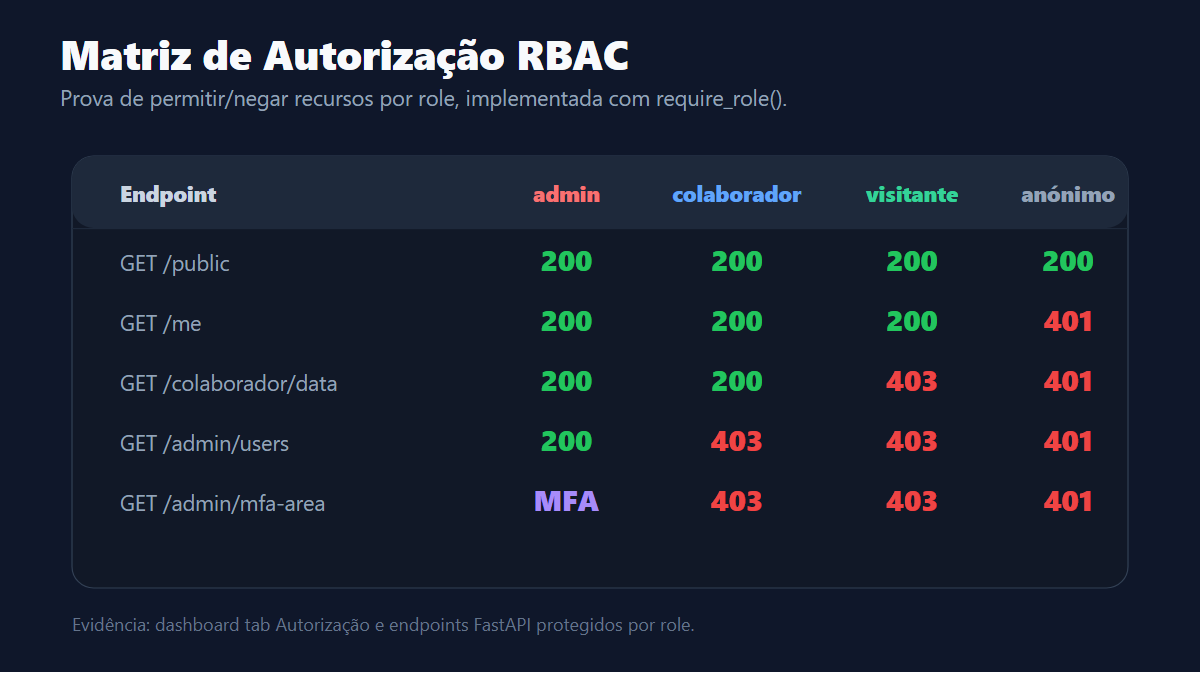
\includegraphics[width=0.95\textwidth]{matriz_rbac.png}
  \caption{Matriz RBAC: mapeamento de endpoints para papéis com resultados esperados (200/403).}
  \label{fig:rbac}
\end{figure}

\subsection{Implementação das Dependências de Autorização}

\begin{table}[h!]
\centering
\caption{Controlo de acesso por endpoint}
\label{tab:endpoints}
\rowcolors{2}{gray!15}{white}
\begin{tabular}{|l|l|c|c|c|}
\hline
\textbf{Endpoint} & \textbf{Proteção} & \textbf{admin} & \textbf{colab.} & \textbf{visit.} \\ \hline
\texttt{GET /public} & Nenhuma & 200 & 200 & 200 \\ \hline
\texttt{GET /me} & JWT válido & 200 & 200 & 200 \\ \hline
\texttt{GET /colaborador/data} & colaborador\textbar{}admin & 200 & 200 & 403 \\ \hline
\texttt{GET /admin/users} & admin & 200 & 403 & 403 \\ \hline
\texttt{GET /admin/audit} & admin & 200 & 403 & 403 \\ \hline
\texttt{GET /admin/mfa-area} & admin + \gls{mfa} & 200* & 403 & 403 \\ \hline
\multicolumn{5}{l}{\footnotesize * apenas se o token incluir \texttt{amr=otp}} \\
\end{tabular}
\end{table}

\begin{lstlisting}[language=Python, caption={Dependências require\_role() e require\_mfa() em auth.py},label={lst:rbac}]
def require_role(*roles: str):
    async def checker(user=Depends(get_current_user)):
        user_roles = user.get("realm_access", {}).get("roles", [])
        if not any(r in user_roles for r in roles):
            raise HTTPException(status_code=403)
        return user
    return checker

def require_mfa():
    async def checker(user=Depends(get_current_user)):
        amr = user.get("amr", [])
        if not any(m in amr for m in ["otp", "mfa", "2fa"]):
            raise HTTPException(status_code=403)
        return user
    return checker
\end{lstlisting}

\section{Autenticação Multifator (MFA/TOTP)}
\label{sec:mfa}

A \gls{mfa} foi implementada com \gls{totp} \cite{RFC6238}, compatível com Google Authenticator, Microsoft Authenticator e Authy.

\subsection{Configuração no Keycloak}

\begin{enumerate}
  \item O fluxo de autenticação \textit{browser} inclui a execução \texttt{auth-otp-form} (obrigatória para o papel \texttt{admin});
  \item O utilizador \texttt{admin.user} tem a \textit{Required Action} \texttt{CONFIGURE\_TOTP} ativa;
  \item No primeiro acesso via \textit{browser}, o Keycloak força a leitura do QR Code e a configuração da aplicação TOTP;
  \item Após configuração, o \gls{jwt} passa a incluir \texttt{"amr": ["otp"]} como prova de segundo fator.
\end{enumerate}

\subsection{Validação na API}

O endpoint \texttt{/admin/mfa-area} exige cumulativamente o papel \texttt{admin} e a \textit{claim} \texttt{amr=otp}. Um token de \texttt{admin.user} obtido via \gls{ropc} (sem \gls{mfa}) retorna \textbf{403}; um token obtido via \textit{browser flow} com \gls{totp} retorna \textbf{200}. Esta separação demonstra que a \gls{api} valida a prova de \gls{mfa} de forma independente do Keycloak.

\section{Ciclo de Vida JML}
\label{sec:jml}

\begin{figure}[h!]
  \centering
  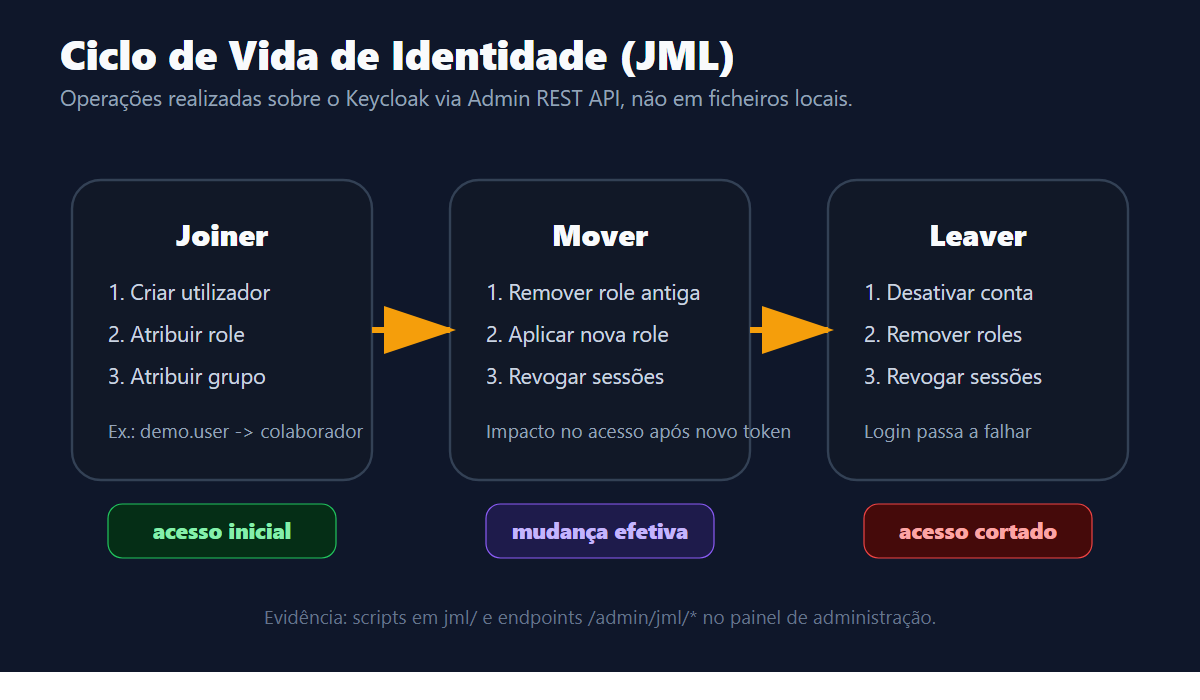
\includegraphics[width=0.95\textwidth]{fluxo_jml.png}
  \caption{Fluxos JML: criação, transição de papel/grupo, desativação e revogação de sessões.}
  \label{fig:jml}
\end{figure}

Os três fluxos foram implementados sobre a Keycloak Admin \gls{rest} \gls{api}, garantindo que toda a gestão de identidades é centralizada no \gls{idp}. Cada fluxo está disponível como script \gls{cli} (\texttt{jml/joiner.py}, \texttt{mover.py}, \texttt{leaver.py}) e como endpoint \gls{rest} (\texttt{POST /admin/jml/\{joiner|mover|leaver\}}).

\begin{table}[h!]
\centering
\caption{Fluxos JML: ações e efeito de segurança imediato}
\label{tab:jml}
\begin{tabularx}{\textwidth}{|l|X|l|}
\hline
\textbf{Fluxo} & \textbf{Ações} & \textbf{Efeito imediato} \\ \hline
Joiner & Cria utilizador, atribui papel e grupo inicial & Acesso inicial controlado \\ \hline
Mover & Troca papel/grupo, \textbf{revoga sessões ativas} & Novo acesso após reautenticação \\ \hline
Leaver & Desativa conta (\texttt{enabled:false}), remove papéis, \textbf{revoga sessões} & Bloqueio imediato de acesso \\ \hline
\end{tabularx}
\end{table}

\subsection{Decisão Técnica: Revogação Explícita de Sessões}

Sem revogação explícita, um utilizador movido ou desativado manteria o acesso durante o tempo de vida do \gls{jwt} (por omissão, 300 segundos). A chamada \texttt{DELETE /admin/realms/iam-tp/users/\{id\}/sessions} força a reautenticação imediata, eliminando esta janela de acesso indevido.

\begin{lstlisting}[language=Python, caption={Revogação de sessões no mover.py},label={lst:revoke}]
# Após trocar papel e grupo:
admin_token = get_admin_token()
user_id = get_user_id(username, admin_token)
revoke_url = f"{KEYCLOAK_URL}/admin/realms/{REALM}/users/{user_id}/sessions"
httpx.delete(revoke_url, headers={"Authorization": f"Bearer {admin_token}"})
\end{lstlisting}

\section{Auditoria de Eventos}
\label{sec:auditoria}

O Keycloak regista automaticamente dois tipos de eventos com persistência em PostgreSQL:

\begin{itemize}
  \item \textbf{Eventos de utilizador}: login, falha de login, logout, \textit{refresh} de token, configuração de \gls{totp} e falhas de \gls{otp};
  \item \textbf{Eventos de administração}: criação/remoção de utilizadores, alteração de papéis e grupos, atualização de clientes.
\end{itemize}

O endpoint \texttt{GET /admin/audit} (protegido por papel \texttt{admin}) agrega ambos os tipos numa única resposta e suporta filtragem por tipo de evento.

\subsection{Excerto de Evidência de Auditoria}

A Listagem~\ref{lst:audit_evento} apresenta um excerto real de evento de login registado pelo Keycloak, tal como retornado pelo endpoint \texttt{/admin/audit}:

\begin{lstlisting}[caption={Excerto de evento de auditoria — login bem-sucedido},label={lst:audit_evento}]
{
  "id": "b3a7c1f2-8d4e-4a2b-9f1c-3e5d7a8b2c4d",
  "time": 1748430600000,
  "type": "LOGIN",
  "realmId": "iam-tp",
  "clientId": "fastapi-client",
  "userId": "a1b2c3d4-e5f6-7890-abcd-ef1234567890",
  "sessionId": "c9d8e7f6-a5b4-3c2d-1e0f-9a8b7c6d5e4f",
  "ipAddress": "172.18.0.1",
  "details": {
    "auth_method": "openid-connect",
    "auth_type": "code",
    "response_type": "code",
    "redirect_uri": "http://localhost:8000/auth/callback",
    "consent": "no_consent_required",
    "code_id": "...",
    "username": "colaborador.user",
    "response_mode": "query"
  }
}
\end{lstlisting}

E um excerto de evento administrativo \gls{jml} (criação de utilizador via Joiner):

\begin{lstlisting}[caption={Excerto de evento de administração — criação de utilizador (Joiner)},label={lst:audit_admin}]
{
  "id": "f4e3d2c1-b0a9-8765-4321-fedcba987654",
  "time": 1748431200000,
  "operationType": "CREATE",
  "resourceType": "USER",
  "realmId": "iam-tp",
  "representation": "{\"username\":\"demo.user\",\"enabled\":true}",
  "resourcePath": "users/f1e2d3c4-a5b6-7890-abcd-ef0123456789",
  "authDetails": {
    "realmId": "iam-tp",
    "clientId": "admin-cli",
    "userId": "admin-service-account",
    "ipAddress": "172.18.0.1"
  }
}
\end{lstlisting}

A evidência consultável completa está disponível no dashboard interativo (aba \textbf{Auditoria}), com filtragem por tipo de evento (\texttt{LOGIN}, \texttt{LOGIN\_ERROR}, \texttt{UPDATE\_TOTP}, etc.) e resumo estatístico por categoria.

\section{Segurança Operacional}

\begin{table}[h!]
\centering
\caption{Riscos identificados e mitigações implementadas}
\label{tab:riscos}
\rowcolors{2}{gray!15}{white}
\begin{tabularx}{\textwidth}{|X|X|}
\hline
\textbf{Risco} & \textbf{Mitigação} \\ \hline
Token inválido ou forjado & Validação RS256 via \gls{jwks}, verificação de \texttt{issuer} e \texttt{audience} \\ \hline
Acesso indevido a recursos & \gls{rbac} no \textit{backend} com \texttt{require\_role()} por endpoint \\ \hline
Administrador sem segundo fator & \gls{totp} obrigatório e validação de \texttt{amr} na \gls{api} \\ \hline
Sessões ativas após mudança de papel & Revogação explícita (\texttt{DELETE /users/\{id\}/sessions}) no Mover e Leaver \\ \hline
Credenciais expostas no código & Variáveis de ambiente via \texttt{.env} (não versionado) \\ \hline
Falta de rastreabilidade & Eventos Keycloak (PostgreSQL) e endpoint \texttt{/admin/audit} protegido \\ \hline
\end{tabularx}
\end{table}

%% ============================================================
%%  Capítulo 5 — Validação e Resultados
%% ============================================================
\chapter{Validação e Resultados}
\label{chap:validacao}

\section{Testes Unitários}

Foram implementados quatro testes unitários em \texttt{tests/test\_auth.py} que validam a lógica central de autenticação e autorização \textbf{sem necessitar de serviços em execução}. Os testes geram um par de chaves RSA temporário para simular as chaves do Keycloak, usando \textit{mocking} de \texttt{\_get\_jwks()}.

\begin{table}[h!]
\centering
\caption{Testes unitários implementados e cobertura}
\label{tab:testes}
\begin{tabularx}{\textwidth}{|l|X|}
\hline
\textbf{Teste} & \textbf{O que valida} \\ \hline
\texttt{test\_require\_role\_allows\_admin} & \texttt{require\_role("admin")} aceita token com papel \texttt{admin} \\ \hline
\texttt{test\_require\_role\_denies\_non\_admin} & Papel incorreto retorna HTTP~403 \\ \hline
\texttt{test\_require\_mfa\_denies\_without\_otp} & Ausência de \texttt{amr=otp} retorna HTTP~403 \\ \hline
\texttt{test\_get\_current\_user\_decodes\_rs256} & Validação de assinatura RS256, \textit{issuer} e \textit{audience} com \gls{jwks} simulado \\ \hline
\end{tabularx}
\end{table}

\begin{lstlisting}[caption={Execução dos testes unitários},label={lst:pytest}]
pip install -r requirements-dev.txt
python -m pytest tests/ -v
# Resultado esperado:
# test_require_role_allows_admin       PASSED
# test_require_role_denies_non_admin   PASSED
# test_require_mfa_denies_without_otp  PASSED
# test_get_current_user_decodes_rs256  PASSED
# 4 passed in 0.XXs
\end{lstlisting}

\section{Validação Funcional via Dashboard}

O dashboard interativo (\texttt{http://localhost:8000/dashboard}) permite validar visualmente todos os requisitos do enunciado sem necessitar de ferramentas externas. A Figura~\ref{fig:dashboard} mostra as abas disponíveis.

\begin{figure}[h!]
  \centering
  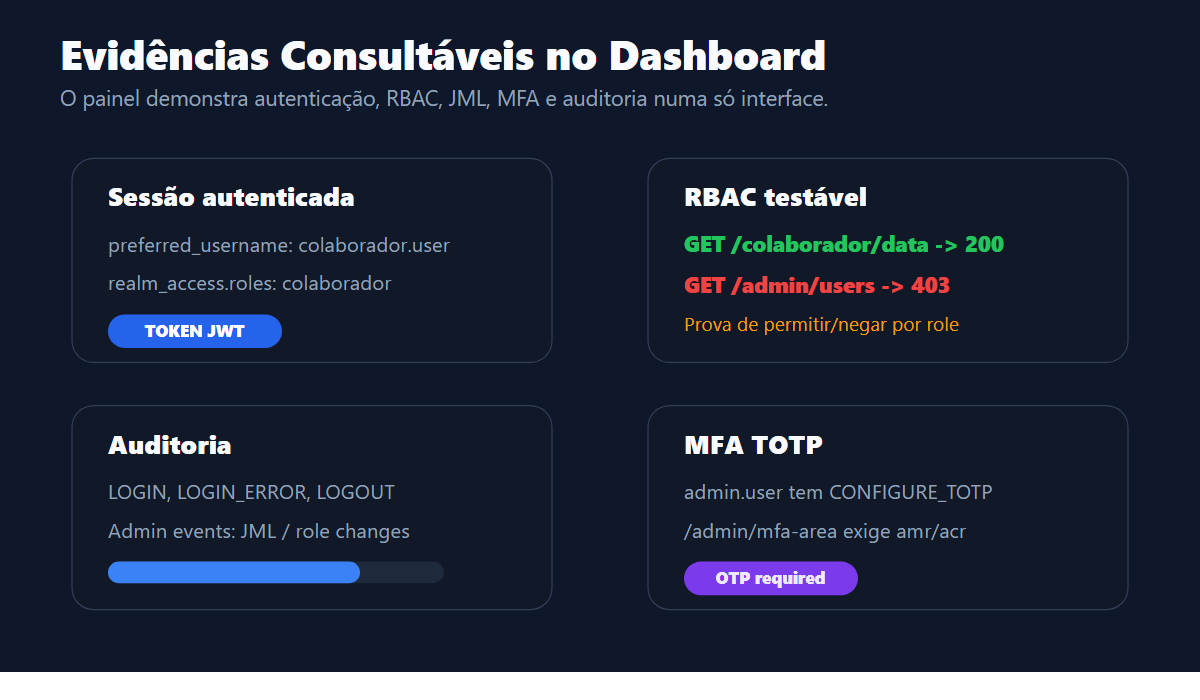
\includegraphics[width=0.95\textwidth]{evidencias_dashboard.png}
  \caption{Dashboard interativo: abas de autenticação, RBAC, JML, auditoria e arquitectura.}
  \label{fig:dashboard}
\end{figure}

O dashboard inclui seis abas de demonstração:

\begin{enumerate}
  \item \textbf{Autenticação} — formulário de login, descodificador de \gls{jwt} com todas as \textit{claims}, \textit{countdown} de expiração;
  \item \textbf{Autorização} — matriz \gls{rbac} com botão \textit{``Testar Todos os Endpoints''}, demonstra respostas 200/403 automaticamente para o utilizador autenticado;
  \item \textbf{JML} — formulários Joiner, Mover e Leaver com chamadas à \gls{api} em tempo real;
  \item \textbf{Auditoria} — lista de eventos filtráveis por tipo, resumo estatístico por categoria, eventos de administração;
  \item \textbf{MFA} — demonstração do fluxo \gls{totp} e validação do endpoint \texttt{/admin/mfa-area};
  \item \textbf{Arquitectura} — diagrama de componentes e mapeamento de portos.
\end{enumerate}

\section{Verificação de Requisitos do Enunciado}

A Tabela~\ref{tab:requisitos} apresenta a verificação de cumprimento de cada requisito do enunciado.

\begin{table}[h!]
\centering
\caption{Verificação de cumprimento dos requisitos do enunciado (Secção 3)}
\label{tab:requisitos}
\rowcolors{2}{gray!15}{white}
\begin{tabularx}{\textwidth}{|X|c|}
\hline
\textbf{Requisito} & \textbf{Estado} \\ \hline
Realm dedicado ao TP (\texttt{iam-tp}) & $\checkmark$ \\ \hline
Estrutura de utilizadores, grupos e papéis no Keycloak & $\checkmark$ \\ \hline
Pelo menos 3 perfis como \textit{realm roles} e \textit{groups} & $\checkmark$ \\ \hline
Login funcional via Keycloak (cliente OIDC \texttt{fastapi-client}) & $\checkmark$ \\ \hline
Validação de sessão/token e \textit{claims} básicas (\texttt{sub}, \texttt{email}, \texttt{roles}) & $\checkmark$ \\ \hline
Prova de controlo de acesso (200/403) por papel com evidência & $\checkmark$ \\ \hline
\gls{mfa} \gls{totp} configurado no Keycloak + zona protegida exige \gls{mfa} & $\checkmark$ \\ \hline
Evidência do fluxo de \textit{setup} e autenticação com \gls{otp} & $\checkmark$ \\ \hline
Joiner: criação de utilizador + atribuição inicial de \textit{groups}/\textit{roles} & $\checkmark$ \\ \hline
Mover: mudança de \textit{group}/\textit{role} com impacto imediato no acesso & $\checkmark$ \\ \hline
Leaver: desativar utilizador, remover \textit{roles} e revogar sessões & $\checkmark$ \\ \hline
Registo de eventos críticos (logins, erros, \gls{mfa}, \gls{jml}) & $\checkmark$ \\ \hline
Evidência consultável com excerto incluído no relatório & $\checkmark$ \\ \hline
\texttt{docker compose up} inicia Keycloak, PostgreSQL e aplicação & $\checkmark$ \\ \hline
\texttt{realm-export.json} para reproduzir configuração & $\checkmark$ \\ \hline
Execução reproduzível (README com passos) & $\checkmark$ \\ \hline
Sem \textit{secrets} \textit{hardcoded} no código & $\checkmark$ \\ \hline
Organização de código e configuração clara & $\checkmark$ \\ \hline
\end{tabularx}
\end{table}

\section{Critérios de Avaliação}

A Tabela~\ref{tab:avaliacao} mapeia os critérios de avaliação do enunciado à evidência disponível na solução.

\begin{table}[h!]
\centering
\caption{Critérios de avaliação (0--20) e evidências correspondentes}
\label{tab:avaliacao}
\begin{tabularx}{\textwidth}{|X|c|X|}
\hline
\textbf{Critério} & \textbf{Peso} & \textbf{Evidência} \\ \hline
Arquitetura e coerência técnica & 20\% & Docker Compose, \texttt{realm-export.json}, separação de serviços \\ \hline
Autenticação / Federação & 15\% & \gls{oidc} via Keycloak, validação \gls{jwt} RS256/\gls{jwks}, dashboard \\ \hline
Autorização & 15\% & \gls{rbac} 3 papéis, \texttt{require\_role()}, matriz 200/403 \\ \hline
\gls{jml} & 15\% & Joiner, Mover, Leaver + revogação imediata de sessões \\ \hline
\gls{mfa} & 15\% & \gls{totp} obrigatório, \texttt{require\_mfa()}, endpoint \texttt{/admin/mfa-area} \\ \hline
Auditoria e segurança operacional & 10\% & Eventos Keycloak, \texttt{/admin/audit}, excerto no relatório \\ \hline
Qualidade da demo e comunicação & 10\% & Dashboard, \texttt{DEMO.md}, guião 10 minutos \\ \hline
\end{tabularx}
\end{table}

%% Capítulo 6 — Conclusão
\chapter{Conclusão}
\label{chap:conclusao}

O projeto implementou com sucesso uma plataforma \gls{iam} completa que cobre todos os requisitos do enunciado. As decisões técnicas mais relevantes foram: (1)~\textbf{validação local de \gls{jwt}} via \gls{jwks} cacheado, que elimina latência e dependência do \gls{idp} em cada pedido; (2)~\textbf{revogação explícita de sessões} no Mover e Leaver, que garante efeito imediato sem aguardar a expiração do token; (3)~\textbf{\textit{realm} declarativo} em \texttt{realm-export.json}, que torna o ambiente completamente reproduzível com um único comando.

Como trabalho futuro identificam-se: substituição do fluxo \gls{ropc} por \textit{Authorization Code + PKCE} na aplicação; rotação automática de chaves \gls{jwks}; suporte a \textit{passkeys}/FIDO2 (AAL3); e exportação de eventos para um \gls{siem} para correlação em tempo real.


%% ---- BIBLIOGRAFIA ----
\bibliographystyle{ieeetr}
\bibliography{refs}

%% ---- ANEXOS ----
\appendix
%% ============================================================
%%  Anexo A — Configuração do Realm Keycloak
%% ============================================================
\chapter{Configuração do Realm Keycloak}
\label{anx:realm}

O ficheiro \texttt{realm-export.json} contém a exportação completa do \textit{realm} \texttt{iam-tp}. Os elementos configurados incluem:

\begin{itemize}
  \item \textbf{Papéis de \textit{realm}}: \texttt{admin}, \texttt{colaborador}, \texttt{visitante};
  \item \textbf{Grupos}: \texttt{/Admins}, \texttt{/Colaboradores}, \texttt{/Visitantes} com mapeamento automático de papéis via \textit{group role mappings};
  \item \textbf{Cliente \gls{oidc}}: \texttt{fastapi-client} com \textit{Authorization Code + PKCE} e \textit{Direct Access Grants} (para testes), \textit{redirect URIs} restritas;
  \item \textbf{Fluxo de autenticação \textit{browser}}: inclui execução \texttt{auth-otp-form} para \gls{mfa};
  \item \textbf{Utilizadores de teste}: \texttt{admin.user}, \texttt{colaborador.user}, \texttt{visitante.user};
  \item \textbf{Configuração de segurança}: RS256, \textit{access token} 300s, \textit{refresh token} 30min.
\end{itemize}

Para reimportar o \textit{realm} (ex.: após destruir os volumes Docker):

\begin{lstlisting}[caption={Reimportação do realm via Docker Compose},label={lst:realm_import}]
# Parar e apagar volumes (dados do Keycloak)
docker compose down -v

# Reiniciar -- o Keycloak importa automaticamente o realm-export.json
docker compose up --build
\end{lstlisting}

Para exportar uma nova versão do \textit{realm} após alterações manuais no Keycloak Admin Console:

\begin{lstlisting}[caption={Exportar realm atualizado},label={lst:realm_export}]
docker compose exec keycloak \
  /opt/keycloak/bin/kc.sh export \
  --dir /tmp/export \
  --realm iam-tp \
  --users realm_file

docker compose cp keycloak:/tmp/export/iam-tp-realm.json ./realm-export.json
\end{lstlisting}

%% ============================================================
%%  Anexo B — Utilizadores de Teste
%% ============================================================
\chapter{Utilizadores de Teste}
\label{anx:utilizadores}

A Tabela~\ref{tab:users} lista os utilizadores pré-configurados no \textit{realm} \texttt{iam-tp} para demonstração.

\begin{table}[h!]
\centering
\caption{Utilizadores de teste do realm \texttt{iam-tp}}
\label{tab:users}
\begin{tabular}{|l|l|l|l|}
\hline
\textbf{Username} & \textbf{Password} & \textbf{Papel} & \textbf{\gls{mfa}} \\ \hline
\texttt{admin.user} & \texttt{Admin@1234} & admin & \gls{totp} obrigatório \\ \hline
\texttt{colaborador.user} & \texttt{Colab@1234} & colaborador & Não configurado \\ \hline
\texttt{visitante.user} & \texttt{Visit@1234} & visitante & Não configurado \\ \hline
\end{tabular}
\end{table}

\textbf{Nota}: estas credenciais são ficcionais e destinam-se exclusivamente a demonstração em ambiente local. Nunca devem ser usadas em ambientes de produção ou em demonstrações com dados reais.

Para criar utilizadores adicionais via \gls{cli}:

\begin{lstlisting}[caption={Criar utilizador via script Joiner},label={lst:joiner_cli}]
python jml/joiner.py \
  --username novo.colaborador \
  --email novo@empresa.pt \
  --role colaborador \
  --password "Senha@2026"
\end{lstlisting}

%% ============================================================
%%  Anexo C — Guião de Demonstração (10 minutos)
%% ============================================================
\chapter{Guião de Demonstração}
\label{anx:demo}

Este anexo resume o guião de demonstração de 10 minutos para a aula final.

\textbf{Pré-requisito}: \texttt{docker compose up} com os três serviços \textit{healthy}.

\begin{table}[h!]
\centering
\caption{Plano de demonstração — 10 minutos}
\label{tab:demo}
\begin{tabularx}{\textwidth}{|c|l|X|}
\hline
\textbf{Tempo} & \textbf{Bloco} & \textbf{Ação / Evidência} \\ \hline
00:00--01:00 & Arranque e Arquitetura & Mostrar logs dos 3 serviços \textit{healthy}; abrir dashboard; apontar diagrama \\ \hline
01:00--03:00 & Autenticação \gls{oidc} & Login \texttt{colaborador.user}; mostrar \gls{jwt} decoded, \textit{claims}, \textit{countdown}; comparar com \texttt{visitante.user} \\ \hline
03:00--04:30 & Autorização \gls{rbac} & Tab Autorização; botão ``Testar Todos''; mostrar 200/403 por papel \\ \hline
04:30--06:00 & \gls{mfa} \gls{totp} & Login \texttt{admin.user} com \gls{totp}; mostrar \texttt{amr:otp}; testar \texttt{/admin/mfa-area} \\ \hline
06:00--08:30 & \gls{jml} & Joiner: criar \texttt{demo.user}; Mover: trocar papel + revogar; Leaver: desativar \\ \hline
08:30--09:30 & Auditoria & Tab Auditoria; filtros \texttt{LOGIN}/\texttt{LOGIN\_ERROR}; eventos admin \gls{jml} \\ \hline
09:30--10:00 & Fecho & Tab Arquitetura; critérios cobertos; testes \texttt{pytest} \\ \hline
\end{tabularx}
\end{table}

O ficheiro \texttt{docs/relatorio/DEMO.md} contém o guião detalhado com as frases de abertura de cada bloco, os passos técnicos e as notas de contingência para situações como Keycloak não disponível ou \gls{totp} desfasado.


\end{document}
